\documentclass{article}

\usepackage{amsmath}
\usepackage{amsthm}
\usepackage{graphicx}


\newtheorem{algorithm}{Algorithm}
\setlength\parindent{0pt}

\title{Group Assignment 1}
\author{Chance Zibolski, Dean Johnson}

\begin{document}
\maketitle

\section*{Problem}
Given an array of small integers $a[1,\ldots,n]$ (that contains a least one
positive integer), compute
\begin{eqnarray*}
  \label{MaxSubArray}
  \max_{i \leq j}\sum_{k=i}^{j}a[k]
\end{eqnarray*}


\begin{algorithm}
\textbf{Enumeration}: Loop over each pair of indices $ i \leq j $ and
compute the sum $\sum_{k=i}^{j}a[k]$
\end{algorithm}

\section*{Psuedocode}

\begin{verbatim}
MaxSubArray(a[1, ..., n])
  max_sum = 0
  sum = 0
  for i = 1, ..., n
    for j = i, ..., n
      for k = i, ..., j
        sum = sum + a[k]
      if sum > max_sum
        max_sum = sum
  return max_sum
\end{verbatim}

\section*{Run-time analysis}

\subsection*{Number of operations}
\begin{eqnarray*}
  \sum_{i=1}^{n}\sum_{j=i}^{n}\sum_{k=i}^{j}a[k]
\end{eqnarray*}

\subsection*{Asymptotic bounds}
\begin{eqnarray*}
    (\mathcal{O}(n^2) \times (\mathcal{O}(n) \text{time to compute each sum})) = \mathcal{O}(n^3)
\end{eqnarray*}

\begin{algorithm}
\textbf{Better Enumeration}: Notice that in the previous algorithm,  the
same sum is computed many times.  In particular, notice that
$\sum_{k=i}^{j}a[k]$ can be computed from $\sum_{k=i}^{j-1}a[k]$ in
$\mathcal{O}(1)$ time, rather than starting from scratch. Write a new version
of the first algorithm that takes advantage of this observation.
\end{algorithm}

\section*{Psuedocode}

\begin{verbatim}
MaxSubArray(a[1, ..., n])
  max_sum = 0
  for i = 1, ..., n
    sum = 0
    for j = i, ..., n
      sum = sum + a[j]
      if sum > max_sum
        max_sum = sum
  return max_sum
\end{verbatim}

\section*{Run-time analysis}

\subsection*{Number of operations}
\begin{eqnarray*}
  \sum_{i=1}^{n}\sum_{j=i}^{n}a[j]
\end{eqnarray*}

\subsection*{Asymptotic bounds}
\begin{eqnarray*}
    ((\mathcal{O}(n) \text{i-iterations}) \times
    (\mathcal{O}(n) \text{j-iterations}) \times
    (\mathcal{O}(n) \text{time to update sum}) ) = \mathcal{O}(n^2)
\end{eqnarray*}


\begin{algorithm}
\textbf{Dynamic Programming}: Your dynamic programming algorithm should be
based on the following idea:

\begin{itemize}
\item The maximum subarray either uses the last element in the input array,
or it doesn't.
\end{itemize}

Describe the solution to the maximum subarray problem recursively and
mathematically based on the above idea.
\end{algorithm}

\section*{Recursive Formula}

\[
  MaxSubArray(a[1, \ldots, n]) =
  \begin{cases}
      MaxSubArray\left(a[1, \ldots, \frac{n}{2}]\right)\\
      MaxSubArray\left(a[\frac{n}{2}, \ldots, n]\right)\\
      MaxSuffix\left(a[1, \ldots, \frac{n}{2}]\right) +
      MaxPrefix\left(a[\frac{n}{2}, \ldots, n]\right)\\
  \end{cases}
\]

\begin{verbatim}
MaxSuffix(a[low, ..., mid])
  max = 0
  sum = 0
  for i = mid, ..., low
    sum = sum + a[i]
    if sum > max
      max = sum
  return max

MaxSuffix(a[mid, ..., high])
  max = 0
  sum = 0
  for i = mid, ..., high
    sum = sum + a[i]
    if sum > max
      max = sum
  return max
\end{verbatim}

\section*{Psuedocode}

\begin{verbatim}
MaxSubArray(a[1, ..., n])
  max = 0
  sum = 0
  for i = 1, ..., n
    sum = sum + a[i]
    if sum < 0
      sum = 0
    if sum > max
      max = sum
  return max
\end{verbatim}

\section*{Run-time analysis}

\subsection*{Number of operations}
\begin{eqnarray*}
  \sum_{i=1}^{n}a[i]
\end{eqnarray*}

\subsection*{Asymptotic bounds}
\begin{eqnarray*}
    (\mathcal{O}(n) \text{i-iterations}) \times
    (\mathcal{O}(c) \text{to compute sum}) = \mathcal{O}(n)
\end{eqnarray*}

\section{Graphs}

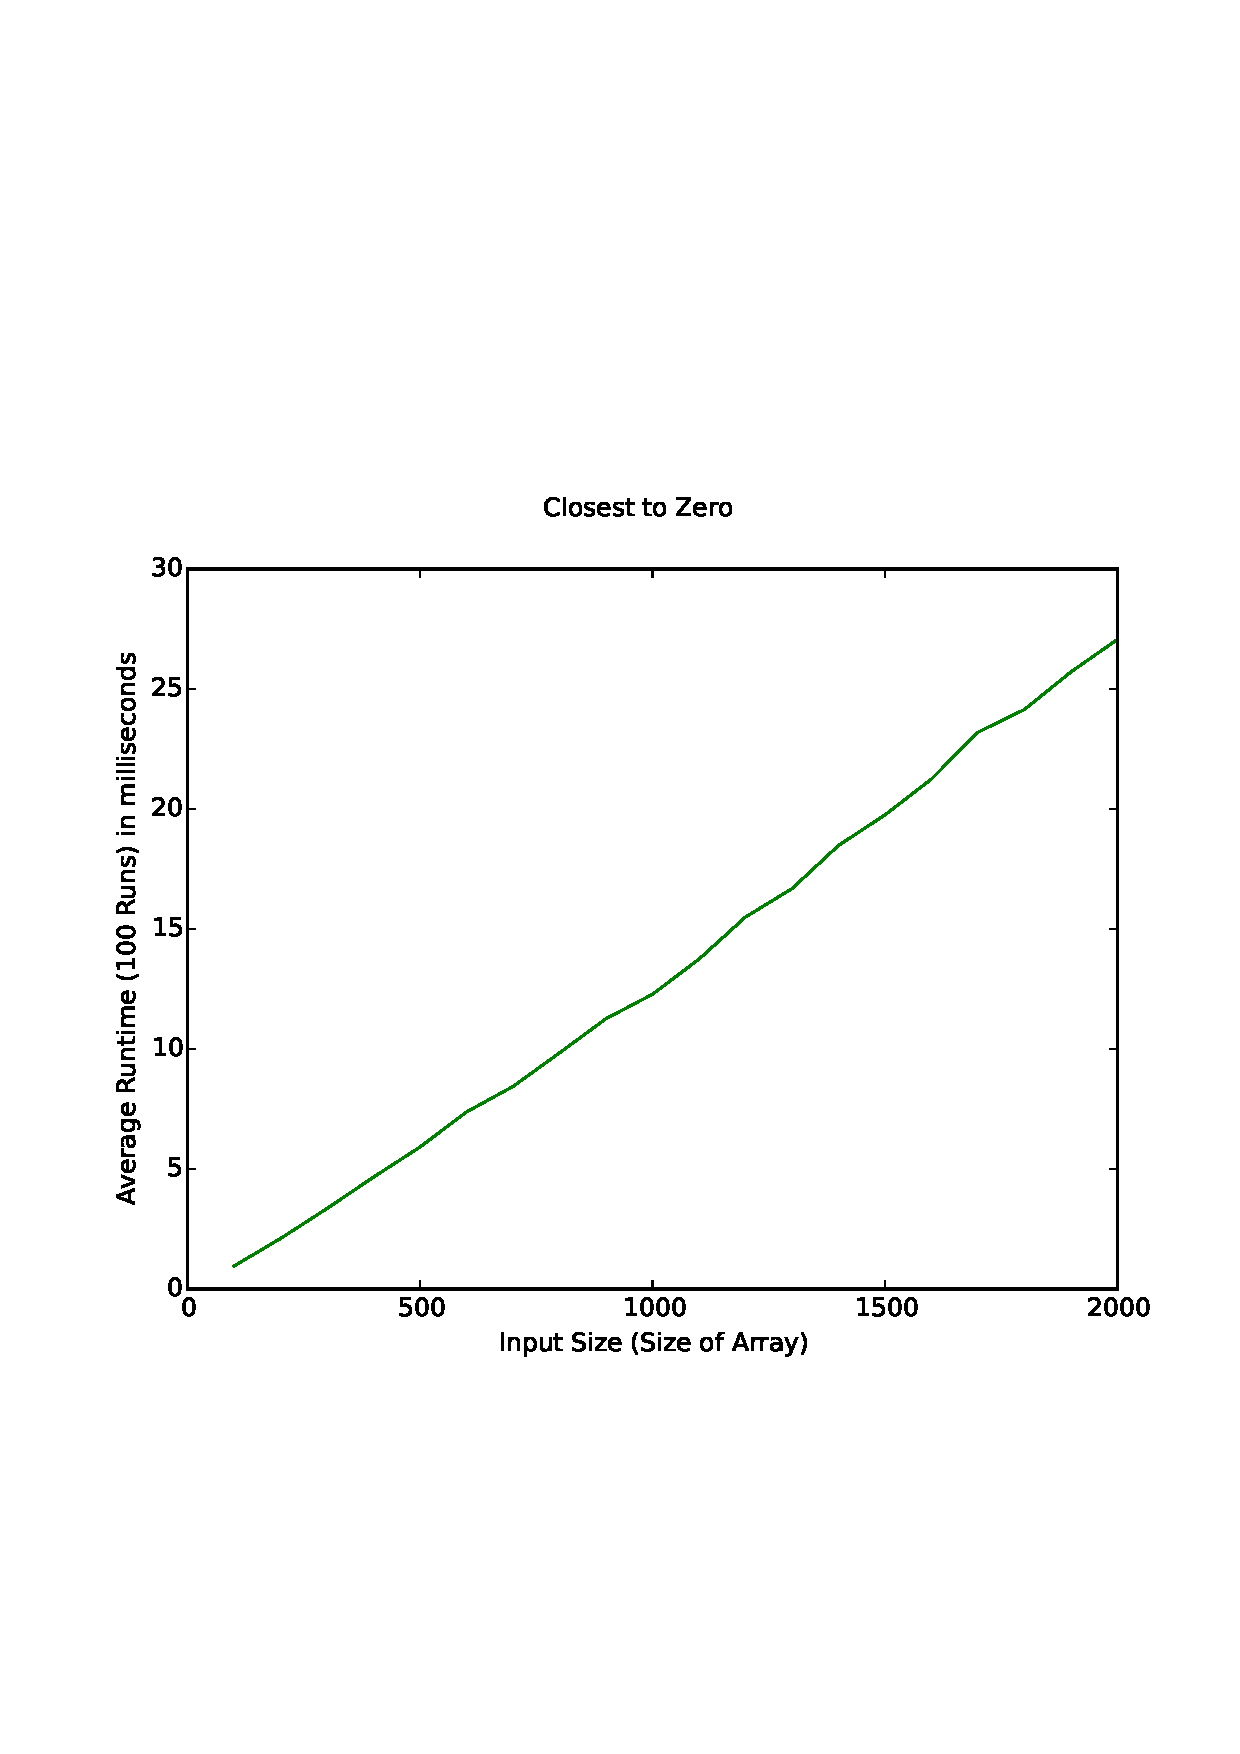
\includegraphics[width=\textwidth]{timings}

\subsubsection*{Slope comparision}

During our experiments we obtained the following slopes for our algorithms:

\begin{itemize}
\item Algorithm 1: 0.3800
\item Algorithm 2: 0.5048
\item Algorithm 3: 1.0050
\end{itemize}

This would give us the following runtime complexity for each algorithm:

\begin{itemize}
    \item Algorithm 1: $\mathcal{\theta}(n^{0.3800})$
    \item Algorithm 2: $\mathcal{\theta}(n^{0.5048})$
    \item Algorithm 3: $\mathcal{\theta}(n^{1.0050})$
\end{itemize}

For our last algorithm, the experimental runtime analysis is accurate to what
our theoretical running time. This accuracy can be attributed to the fact that
the algorithms linear runtime and the ease of implementation compared to the
other algorithms.

The enumeration and better enumeration algorithms, (1 and 2) both had lower
runtime complexities when measured than what we would expect. For algorithm 1
we expected a runtime complexity of $\mathcal{\theta}(n^3)$ but instead ended
up with $0.3800$ which could be caused by our experimental data being so small.
The second algorithm we expected to run in $\mathcal{\theta}(n^2)$ time, but it
actually ended up taking $\mathcal{\theta}(n^{\frac{1}{2}})$ which suggests we
may have made an error when measuring our data, or the algorithm is wrong.
However, the algorithm looks fundamentally correct, so I would attribute the
error to the experimental data, and inconsistencies caused by computer caching,
and such.

\end{document}
